\noindent Podle Schaumanna a Valkenburga \cite{13} je pro ideální OTA zesilovač (vstupní i výstupní impedance nulové) možno odpor nahradit obvodem s uzemněným neinvertujícím vstupem a zpětnou vazbou z invertujícího vstupu na výstup a to hodnotou
\begin{align}
R_{in} = \frac{1}{g_{m}},
\end{align}
kde $g_{m}$ označuje transkonduktanci zesilovače. Prohození invertujícího a neinvertujícího vstupu vede na opačnou polaritu. Tato konfigurace jako odpor je užitečná např. k návrhu monolitických $g_m$-C filtrů pouze s transkonduktancemi a kapacitami ($g_m$-C filtry, viz \ref{s:OTA}, \ref{s:GM-C}), také k náhradě velmi velkých odporů.
\begin{figure}[h]
\centering
\includegraphics[scale=0.4]{image10.png}
\caption[Náhradní obvod pro uzemněný rezistor]{Náhradní obvod pro uzemněný rezistor}
\end{figure}
\noindent Dále lze dle Schaumanna a Valkenburga~\cite{13} pro nahrazení indukčnosti o impedanci $Z_L = 1/(pC)$ použít obvod se~třemi OTA (obrázek~\ref{s:IND0}). Uzemněny jsou invertující vstup prvního OTA a neinvertující druhého. Použita je zpětná vazba z výstupu na neinvertující vstup prvního OTA. Propojení výstupu prvního OTA na invertující vstup druhého OTA je realizován přes uzemněný kapacitor. \\
Vyjádřením napětí a proudů v obvodu bylo získáno napětí na kapacitoru a vstupní proud
\begin{align}\label{s:vzt2}
V_C &= \frac{g_{m1}}{sC}V_1, \\
I_1 &= g_{m2}V_C = \frac{g_{m1}g_{m2}}{pC}V_1.
\end{align}
Výsledná indukčnost --- impedance vstupu byla vyjádřena vztahem \ref{s:vzt2}.
\begin{align}
Z_{in}(p) = \frac{V_1}{I_1} = p\frac{C}{g_{m1}g_{m2}}
\end{align}
\noindent Byl obdržen induktor o hodnotě
\begin{align}
L = \frac{C}{g_{m1}g_{m2}}.
\end{align}
\begin{figure}[h]
\centering
\includegraphics[scale=0.4]{image12.png}
\caption[Náhradní obvod pro neuzemněnou indukčnost]{Náhradní obvod pro neuzemněnou indukčnost pro $g_{m1} = g_{m2}$ \label{s:IND0}}
\end{figure}
\begin{figure}[h]
\centering
\includegraphics[scale=0.4]{image13.png}
\caption[Náhradní obvod pro indukčnost]{Náhradní obvod pro indukčnost \label{s:IND}}
\end{figure}
\\
\noindent Pro uzemněnou indukčnost o impedanci $Z_L = 1/(pC)$ byl podle Schaumanna a Valkenburga \cite{13} použit obvod na obrázku \ref{s:IND}. Vyjádřením napětí a proudů v obvodu bylo získáno napětí na kapacitoru a vstupní proud
\begin{align}
V_C &= \frac{g_{m1}}{pC}V_1, \\
I_1 &= g_{m2}V_C = \frac{g_{m1}g_{m2}}{pC}V_1.
\end{align}
Výsledná indukčnost --- impedance vstupu byla vyjádřena vztahem
\begin{align}
Z_{in}(p) = \frac{V_1}{I_1} = p\frac{C}{g_{m1}g_{m2}}.
\end{align}
\subsection{Základní bloky}
\begin{figure}[h]
\centering
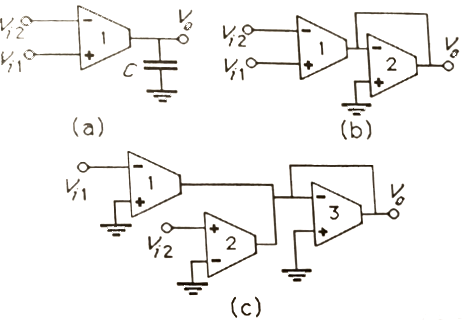
\includegraphics[scale=0.4]{otos.png}
\caption[Základní bloky s OTA]{Základní bloky s OTA a) integrující b) škálující c) sčítací \label{s:BLO}}
\end{figure}
\noindent Podle Schaumanna a Valkenburga \cite{13} blok a) na obrázku \ref{s:BLO} slouží k realizaci invertujícího nebo neinvertujícího integrátoru s~výsledným napětím
\begin{equation}
V_O = \frac{g_{m1}}{pC}(V_1 - V_2).
\end{equation}
Blok b) na obrázku \ref{s:BLO} je komparátor s různou polaritou a napětím na výstupu
\begin{equation}
V_O = \frac{g_{m1}}{g_{m2}}(V_1 - V_2).
\end{equation}
Blok c) na obrázku \ref{s:BLO} realizuje sčítací nebo rozdílový obvod s napětím na výstupu
\begin{equation}
V_O = -\frac{g_{m1}}{g_{m3}}V_1 + \frac{g_{m2}}{g_{m3}}V_2.\label{s:BLO3}
\end{equation}
\noindent Spojením těchto základních stavebních bloků se správnými znaménky lze získat různé funkční bloky.\\
Základním principem uplatňovaným při návrhu s OTA je použití pouze OTA a uzemněných kapacitorů, protože při návrhu IC jsou uzemněné kapacitory méně zatíženy parazitními chybami než neuzemněné kapacitory. Pro IC použití je vhodné volit shodné transkonduktance. Parazitní vstupní a především výstupní impedance způsobují chyby ve výstupu filtru, což může vést na parazitní póly, které při vysokofrekvenčním použití nelze zanedbat. Při použití filtru pro zvukové aplikace (20--20 000\,Hz) naopak lze chyby způsobené parazitními součástkami i~chyby způsobené konečnou šířkou pásma zanedbat.
\subsection{Odvození DP 2. řádu}\label{s:ODV}
\noindent Náhradní obvod, ze kterého bude spočítána přenosová funkce pro přenos filtru druhého řádu, popisuje obrázek~\ref{s:DPO}.
\begin{figure}[h]
\centering
\includegraphics[scale=0.3]{circuit(2).png}
\caption{Dolní propust 2. řádu \label{s:DPO}} 
\end{figure}
\noindent Přenos obvodu byl vyjádřen jako
\begin{align}
H(p) = \frac{U_{out}}{U_{in}} = \frac{Z_2}{Z_1}, \quad Z_1 = pL,\quad Z_2 = \frac{\frac{R}{pC}}{R + \frac{1}{pC}}.
\end{align}
Výsledný přenos je roven 
\begin{align}
H(p) = \frac{\frac{\frac{R}{pC}}{R + \frac{1}{pC}}}{pL + \frac{\frac{R}{pC}}{R + \frac{1}{pC}}}.
\end{align}
Elementárními algebraickými úpravami a následným vynásobením členem $1/(LRC)$ byl získán výsledný přenos.
\begin{align}\label{s:vzt4}
H(p) = \frac{R}{p^2LRC + pL + R} = \frac{\frac{1}{LC}}{p^2 + \frac{p}{RC} + \frac{1}{LC}}.
\end{align}
\noindent Využitím poznatků ze sekce \ref{s:NAH} je možno za odpor a indukčnost dosadit do vztahu \ref{s:vzt4}. Byly uvažovány kapacitory o stejné hodnotě C.
\begin{align}
H(p) = \frac{\frac{1}{\frac{C^2}{g_{m1}g_{m2}}}}{p^2 + \frac{p}{\frac{C}{g_{m2}}} + \frac{1}{\frac{C^2}{g_{m1}g_{m2}}}} = \frac{\frac{g_{m1}g_{m2}}{C^2}}{p^2 + \frac{pg_{m2}}{C} + \frac{g_{m1}g_{m2}}{C^2}} = \frac{g_{m1}g_{m2}}{p^2C^2 + pg_{m2}C + g_{m1}g_{m2}}.
\end{align}
Porovnáním jmenovatele se jmenovatelem přenosu filtru 2. řádu byl obdržen vztah
\begin{align}
p^2 + p\frac{\omega _0}{Q} + \omega _0^2 &= p^2C^2 + pg_{m2}C + g_{m1}g_{m2},\\
p^2 + p\frac{\omega _0}{Q} + \omega _0^2 &= p^2 + \frac{pg_{m2}}{C} + \frac{g_{m1}g_{m2}}{C^2}.
\end{align}
Z tohoto vztahu byl vyjádřen mezní kmitočet jako 
\begin{align}
\omega _0^2 &= \frac{g_{m1}g_{m2}}{C^2}, \\
\omega _0 &= \sqrt{\frac{g_{m1}g_{m2}}{C^2}}
\end{align}
a činitel jakosti dosazením za $\omega _0$
\begin{align}
Q = \frac{\omega _0}{\frac{g_{m2}}{C}} = \sqrt{\frac{g_{m1}}{g_{m2}}}.
\end{align}
Pokud navíc byly uvažovány stejné transkonduktance $g_{m1}, \ g_{m2} = g_m$, byl obdržen výsledek
\begin{align}
\omega _0 &= \sqrt{\frac{g_m^2}{C^2}},\\
Q &= \sqrt{1} = 1.
\end{align}